% !TeX root = ../thuthesis-example.tex

\chapter{固体火箭发动机装药设计具体步骤}

\section{药型选择}

与其他类型的药形相比,星形药具有独特的特性。这种药柱可以通过调整星角的大小来实现减面性、恒面性或增面性。此外,还可以通过改变肉厚系数和星孔的几何参数来调整其装填系数。这使得星形药柱能够同时满足恒面燃烧的要求,并具备较高的装填系数,因此它在长时间运行和高推力的发动机中得到了广泛应用。

\section{推进剂种类的选择}

HTPB/AP/Al推进剂具有较大的比冲并且燃速压力指数适中燃烧不是很大更易于控制,同时密度较大,能量特性优异,力学性能优越。因此,HTPB/AP/Al是固体火箭发动机设计中理想的推进剂选择。

下表为HTPB/AP/Al推进剂具体参数

\begin{longtable}{ccc}
    \caption{推进剂参数预选表}
    \label{tab:longtable} \\
    \toprule
    物理量 & 物理量参数 & 数值  \\
    \midrule
  \endfirsthead
    \caption*{续表~\thetable\quad 推进剂参数预选表} \\
    \toprule
    物理量 & 物理量参数 & 数值 \\
    \midrule
  \endhead
    \bottomrule
  \endfoot
  \multirow{4}*{装药几何参数}    & 外径$D$ & 265mm  \\
  & 总冲$I$ &  260$\mathrm{KN}\cdot \mathrm{s}$    \\
  & 平均推力    & 40kN   \\
  & 工作环境温度  & 20 $ ^{\circ} \mathrm{C}$     \\
  \hline
发动机平均工作压力 & 压力值(Mpa)  & 6.9MPa       \\
\hline
环境大气压力    &  压力值(pa) & 101325pa  \\ 
\hline
\multirow{8}*{\begin{tabular}[c]{@{}c@{}}推进剂\\HTPB/AP/Al\end{tabular}}       & 燃气绝热指数  & 1.19   \\
  & 燃气分子量   & 22.3   \\
  & 理论比冲(秒) & 263    \\
  & 火焰温度    & 3150   \\
  & 密度      & 1.77   \\
  & 铝粉含量    & 13     \\
  & 燃速      & 8      \\
  & 燃速压力指数  & 0.33   \\
  & 加工方式    & 浇筑  
\end{longtable}

\section{设计计算步骤}

如下图所示,星型药柱需要确定的几何物理量有药柱外径$D$、药柱内厚$e_{1}$、药柱长度$L$、星型角数$n^{*}$、角系数$\varepsilon $、星边夹角$\theta $、过渡圆弧半径$r$、星角圆弧半径$r_{1}$等参数。

\begin{figure}
  \centering
  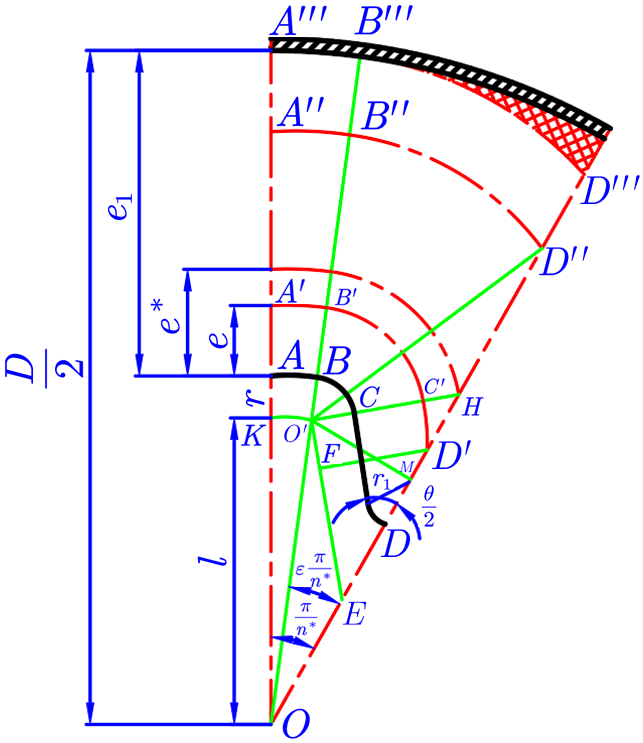
\includegraphics[width=0.6\linewidth]{star.png}
  \caption{星角图}
  \label{fig:star}
\end{figure}

\section{装药量$m_{peff}$}

由规定总冲$I$,求出装药量$m_{peff}$。查阅资料可得发动机制造行过程中会出现各种各样的偏差,导致发动机的性能也产生了不同程度的偏差。为保证达到规定的性能指标,必须对原始数据进行修正。查阅资料可得总冲的相对偏差的3倍值$3\sigma $ / $\overline{x}$一般不大于1\%,于是在发动机初步设计时可以近似地取总冲量的设计值$I_{d}=(1.01\sim 1.05)I$。装药量计算得
\[
  m_{peff}=\frac{(1.01\sim 1.05)I}{gI_{sp}}
  \]
  \[
m_{peff}=\frac{1.03\times 260\times 10^3}{9.8\times 263}=103.903 m/s^2
\]

$I$——总冲量

$g$——重力加速度,取$9.8m/s^{2}$

$I_{sp}$——推进剂比冲

$m_{peff}$——装药量

\section{喷喉面积$A_{t}$}

由于我们现在知道工作压力为6.9MPa时的推进剂燃速,于是我们选取平均工作压力$P_{c}=6.9$MPa。

HTPB的k值为1.19,假设喷管完全膨胀,即$P_{a}=P_{e}=101325pa$。

燃气比热比函数:
\[\Gamma =\sqrt{k}\bigl( \frac{2}{k+1} \bigr) ^{\frac{k+1}{2\left( k-1 \right)}}=\sqrt{1.19}\bigl( \frac{2}{1.19+1} \bigr) ^{\frac{1.19+1}{2\left( 1.19-1 \right)}}=0.647
\]

推力系数:
\[
C_{_F}=\Gamma \sqrt{\frac{2k}{k-1}(1-(\frac{P_e}{P_c})^{\frac{k-1}{k}})}=0.647\times \sqrt{\frac{2\times 1.19}{1.19-1}(1-(\frac{101325}{6.9\times 10^6})^{\frac{1.19-1}{1.19}})}=1.603
\]

喷管喉部面积:
\[
  A_t=F/\left( C_FP_F \right) =\frac{40\times 10^3}{1.603\times 6.9\times 10^6}=0.0036164m^2
\]

此时:
\[
  C^*=I_{sp}g/C_F=1607.860m/s
\]

$k$——燃气绝热指数

$\Gamma$——燃气比热比函数

$P_{e}$——外界大气压强

$P_{c}$——工作压力/燃烧室压力

$C_{F}$——推力系数

\section{平均燃面$\overline{S}$}

常温下的燃速系数,其中常温下燃速压力指数$n_{+20^\circ C}=0.33$:
\[
a_{+20^{\circ}C}=r_{\text{燃}}/\overline{P}_{+20^\circ C}^{n_{+20^\circ C}}=\frac{8.0\times 10^{-3}}{\left( 6.9\times 10^{6} \right) ^{0.33}}=4.4286\times 10^{-5}
\]

常温下特征速度:
\[
  C_{+20^{\circ}\mathrm{C}}^{*}=C^*=1607.86m/s
\]

平均燃面:
\[
\overline{K}_N=\frac{\overline{S}}{A_t}=\frac{\overline{p}_{+20^\circ C}^{1-n_{+20^\circ C}}}{C_{{+20^{\circ}\mathrm{C}}}^{*}\rho {_p}a_{+20^{\circ}\mathrm{C}}}
\]
\[
  \overline{K}_N=\frac{\overline{p}_{+20^\circ C}^{1-n_{+20^\circ C}}}{C_{{+20^{\circ}\mathrm{C}}}^{*}\rho {_p}a_{+20^{\circ}\mathrm{C}}}=\frac{(6.9\times 10^6)^{1-0.33}}{1607.860\times 1.77\times 10^3\times 4.429\times 10^{-5}}=303.041
\]

燃烧面积:
\[
  \overline{S}=\overline{K_N}A_t=303.041\times 0.0036164=1.096m^{2}
\]

$\overline{K_N}$——面喉比

$\overline{S}$——平均燃面

$A_{t}$——喷管喉部面积

$\overline{p_{^\circ C}}$——常温下平均工作压力

$n_{^\circ C}$——常温下燃速压力指数

$C_{+20^{\circ}\mathrm{C}}^{*}$——常温下特征速度

$\rho_{p}$——推进剂密度

$a_{^\circ C}$——常温下的燃速指数

\section{肉厚$e_{1}$}
\[
e_1=\frac{m_{peff}}{\rho _p\bar{S}}=\frac{103.903}{1.77\times 1.096}\times 10^{-3}=0.05356m=53.56mm
\]

$e_{1}$——肉厚

$\rho _{p}$——推进剂密度

$\overline{S}$——平均燃面面积

$m_{peff}$——有效装药量

\section{星角圆弧半径$r_{1}$}

星孔内尖角使用倒角圆化之后,初始燃烧面积减小,最大燃烧面积也减小并向后推迟。若无侵蚀燃烧时,燃烧初期压力曲线将会有一升高阶段。我们想利用侵蚀燃烧将压力曲线补平临界通气参量燃通比$\varphi^*$是判断侵蚀燃烧是否发生的依据,由$J=\varphi/K_N$可得出临界面喉比$J^*=0.2046$,目前已知条件我们无法给出$r_{1}$,因此我们先假设$r_{1}=8mm$,由最后结果侵蚀燃烧的补平情况修正。

\section{选取过渡圆弧半径$r$}
已知$r$增大,应力集中系数降低。但是$r$增大,装填系数降低,因此$r$值应选取适当。
通常:
\[
\overline{r}=\frac{r}{D}=0.015\sim 0.030
\]

这里我们选取0.015
\[
  r=0.015D=0.015\times 265=3.975mm
\]

\section{星角数}

取$n^*$为3、4、5、6、7、8。

\section{特征长度$l$、$y_{0}$、$y_{1}$}
\[
l=\frac{D}{2}-e_1-r=\frac{265}{2}-53.56-3.975=74.965mm
\]
\[
y_0=\frac{r}{l}=\frac{3.975}{74.965}=0.052
\]
\[
y_1=\frac{e_1+r}{l}=\frac{53.56+3.975}{74.965}=0.7675
\]

\section{角度系数\texorpdfstring{$\varepsilon $}{}}

对于星边消失后有:
\[
\left( \frac{s}{l} \right) _{\min}=2n^*\left[ \frac{\sin \varepsilon \frac{\pi}{n^*}}{\sin \frac{\overline{\theta }}{2}}+(1-\varepsilon )\frac{\pi}{n^*} \right] 
\]

选取角度系数$0.3< \varepsilon <0.8$,要求
\[
\xi _2\leqslant 1.2  \hspace{1em}(1)
\]
\[
\xi _2=\frac{\left( \frac{S}{l} \right) _1}{\left( \frac{S}{l} \right) _{\min}}\le 1.2
\]

这里$y_{1}$足够大,所以有:
\[
  \left( \frac{S}{l} \right) _1=2\pi(1+y_{1})
\]

${\left( \frac{S}{l} \right) _{\min}}$——最小无量纲周边长

\vspace{0.8em}
$\xi _2$——增面比

$s$——药柱燃烧周边长

$n^*$——星角数

$\overline{\theta}$——恒面燃烧时对应的星边夹角,只与星角数有关

$\overline{\theta}$可由下式得到:
\[
\frac{\pi}{2}+\frac{\pi}{n^*}-\frac{\overline{\theta }}{2}-\cot \frac{\overline{\theta }}{2}=0
\]

星边消失后需要保证
\[
\sin\mathrm{(}\varepsilon \frac{\pi}{n})/y_1\leqslant 1\hspace{1em}(2)
\]

\section{星角\texorpdfstring{$\theta$}{}}

为了获取平稳的推力曲线,通常希望前期的减面比与后期的增面比满足:
\[
\xi _1\xi _2=1
\]

同时根据选定的$\xi$求得$\xi_{1}$后再求出$\left( \frac{S}{l} \right) _{\max}$:
\[
\xi _1=\frac{\left( \frac{S}{l} \right) _{\min}}{\left( \frac{S}{l} \right) _{\max}}
\]

最后求出星角$\theta /2$:
\begingroup
\fontsize{16}{14}\selectfont 
\[
\left( \tfrac{s}{l} \right) _{r_1}=\left( \tfrac{s}{l} \right) _{max}=2n^*\left[ \tfrac{\sin \left( \varepsilon \frac{\pi}{n^*} \right)}{\sin \frac{\theta}{2}}+\left( 1-\varepsilon \right) \tfrac{\pi}{n^*}+\tfrac{r_1+r}{l}\left( \tfrac{\pi}{2}+\tfrac{\pi}{n^*}-\tfrac{\theta}{2}-\cot\tfrac{\theta}{2} \right) \right] 
\]
\endgroup
\section{通气面积$A_{p}$、通气参量$J$、装填系数\texorpdfstring{$\varepsilon$}{}}

\begingroup
\fontsize{16}{14}\selectfont 

\[
  \begin{array}{ccl}
    \frac{A_p}{l^2}&		=&		n^*\left[ \left( 1-\varepsilon \right) \frac{\pi}{n^*}+\sin \varepsilon \frac{\pi}{n^*}\left( \cos \varepsilon \frac{\pi}{n^*}-\sin \varepsilon \frac{\pi}{n^*}\cdot \cos \frac{\theta}{2} \right) \right]\\[1em]
    &		&		+2n^{^*}y_{_0}\left[ \frac{\sin \varepsilon \frac{\pi}{n^{^*}}}{\sin \frac{\theta}{2}}+(1-\varepsilon )\frac{\pi}{n^{^*}} \right] +ny_{_0}^{2}\left( \frac{\pi}{2}+\frac{\pi}{n^{^*}}-\frac{\theta}{2}-ctg\frac{\theta}{2} \right)\\[1em]
    &		&		+n^*\left( \frac{r_1}{l} \right) ^2\left( \frac{\theta}{2}+ctg\frac{\theta}{2}-\frac{\pi}{2} \right)\\
  \end{array}
  \]

\endgroup

\[
J=\frac{A_{t}}{A_{p}}
\]
\[
  \eta =\frac{A_c-A_p}{A_c}
\]

$A_{p}$——通气面积

$A_{T}$——喷管喉部面积

$A_{c}$——燃烧室横截面积

$n^*$——星角数

$\theta$——星边夹角

$J$——喉通比

$\eta$——装填系数

要求,$0.75\leqslant \eta \leqslant 0.85$\hspace{1em}(3)

\section{剩药面积$A_{f}$、剩药面积\texorpdfstring{$\eta_{f}$}{}}
\begingroup
\fontsize{16}{14}\selectfont 
\[
  \begin{array}{ccl}
    \frac{A_f}{l^2}&		=&		\varepsilon \pi \left( 1+y_1 \right) ^2-n^*\left[ \sin \varepsilon \frac{\pi}{n^*}\left( \sqrt{y_{1}^{2}-\sin ^2\varepsilon \frac{\pi}{n^*}}+\cos \varepsilon \frac{\pi}{n^*} \right) \right]\\[1.5em]
    &		&		-n^*y_{1}^{2}\left[ \varepsilon \frac{\pi}{n^*}+\arcsin\left( \frac{\sin \varepsilon \frac{\pi}{n^*}}{y_1} \right) \right]\\
  \end{array}\]
  \endgroup
\[
\eta _f=\frac{A_f}{A_c}
\]

$A_{f}$——剩药面积

$A_{c}$——药柱横截面积

$l$——特征长度

$\varepsilon$——角度系数

$n^*$——星角数

$\eta_{f}$——剩药系数

要求,$\eta _f\leqslant5\%$\hspace{1em}(4)

  \section{装药长度$L$}
\[
L=\frac{\frac{m_{peff}}{\rho _p}}{A_c-A_p-A_f}
\]

$L$——药柱长度

$m_{peff}$——有效装药量

$\rho_{p}$——推进剂密度

$A_{c}$——药柱横截面积

$A_{p}$——通气面积

$A_{f}$——剩药面积

要求,$1.3m\leqslant L\leqslant 1.8m$\hspace{1em}(5)

\section{燃烧面积$S$}
前期最大无量纲周边长:

\begingroup
\fontsize{16}{14}\selectfont 
\[\left( \frac{s}{l} \right) _{r_1}=2n^*\left[ \frac{\sin \varepsilon \frac{\pi}{n^*}}{\sin \frac{\theta}{2}}+(1-\varepsilon )\frac{\pi}{n^*}+\frac{r+r_{_1}}{l}\left( \frac{\pi}{2}+\frac{\pi}{n^*}-\frac{\theta}{2}-\cot \frac{\theta}{2} \right) \right] 
\]
\endgroup

\vspace{1em}
燃烧初始瞬间无量纲周边长:

\begingroup
\fontsize{16}{14}\selectfont 
\[\left( \frac{s}{l} \right) _0=2n^*\left[ \frac{\sin \varepsilon \frac{\pi}{n^*}}{\sin \frac{\theta}{2}}+(1-\varepsilon )\frac{\pi}{n^*}+\frac{r+r_1}{l}\left( \frac{\pi}{2}+\frac{\pi}{n^*}-\frac{\theta}{2}-\cot \frac{\theta}{2} \right) -\frac{\pi r_1}{n^*l} \right] 
\]
\endgroup
\vspace{1em}

星边消失点无量纲周边长:

\begingroup
\fontsize{16}{14}\selectfont 
\[
\left( \frac{s}{l} \right) ^*=2n^*\left[ \frac{\sin \varepsilon \frac{\pi}{n^*}}{\sin \frac{\theta}{2}}+(1-\varepsilon )\frac{\pi}{n^*}+y^*\left( \frac{\pi}{2}+\frac{\pi}{n^*}-\frac{\theta}{2}-\cot \frac{\theta}{2} \right) \right] 
\]
\endgroup
\vspace{1em}

$n^*$——星角数

$\varepsilon$——角度系数

$\theta$——星边夹角

$l$——特征长度

$r_{1}$——星角圆弧半径

$y^*$———星边消失点无量纲燃层厚度

\begingroup
\fontsize{16}{14}\selectfont 
\[
y^*=\frac{e^*+r}{l}=\frac{\sin \varepsilon \frac{\pi}{n^*}}{\cos \frac{\theta}{2}}
\]
\endgroup